%!TEX root = ../thesis.tex
% створюємо розділ
\chapter{Підготовка до проведення дослідження}
\label{chap:theory}

В даному розділі знаходиться огляд основних інструментів та методів аналізу та попередньої обробки даних, також ми зазначимо використані інструменти та ресурси для моделювання.

\section{Використані інструменти та ресурси}

В якості мови програмування було вибрано Python v3.11~\cite{ct18}, це ефективна та гнучка мова програмування, для розв'язання задач машинного навчання, для якої створено велику кількість бібіліотек та ресурсів, які дозволяють ефективно розв'язувати задачі, включаючи задачі бінарної та багатокласової класифікації табличних даних та картинок. Основними бібліотеками для створення моделей були бібліотеки Deap v1.4~\cite{ct19} та scikit-learn v1.4~\cite{20}. Обидві бібліотеки надають документацію, невеликі навчальні посібники та приклади для пришвидшення побудови моделей.

Бібліотека Deap --- це спеціалізована бібліотека для створення еволюційних алгоритмів. Ця бібліотека має реалізовані рішення для різних задач, таких як генетичне програмування, еволюційні стратегії, генетичні алгоритми та багато інших. Вона забезпечує зручний інтерфейс для налаштування та запуску еволюційних експериментів, надаючи широкий набір інструментів для маніпуляції популяціями, відбору, кросинговеру та мутацій. Основними елементами бібліотеки Deap є індивідуми, популяції, фітнес-функції, оператори генетичних алгоритмів, такі як, відбір, кросинговер та мутація. Ця бібліотека також дозволяє налаштовувати багато параметрів, таких як розмір популяції, кількість поколінь, ймовірності мутацій та кросинговеру, що робить її дуже гнучкою для різних задач. Вона підтримує паралельні обчислення, що значно прискорює процес еволюційного пошуку оптимальних рішень. В даному дослідженні буде використовуватись бібліотека Deap для реалізації $(1+\lambda)$-EA with GP encodings, що дозволяє досліджувати ефективність та керованість цього алгоритму в контексті задачі класифікації. Зокрема, ми будемо використовувати такі оператори, як турнірний відбір та одноточкову мутацію. Крім того, буде проведено аналіз впливу різних гіперпараметрів, таких як, значення $\lambda$ та глибина дерева, а також множини термінальних та внутрішніх вузлів, на якість розв'язків та швидкість конвергенції алгоритму.

Бібліотека scikit-learn --- це популярна бібліотека для машинного навчання, яка надає великий набір інструментів для задач класифікації, регресії, кластеризації, зниження розмірності та попередньої обробки даних. Вона забезпечує простий і уніфікований інтерфейс для побудови та оцінки моделей машинного навчання, що дозволяє швидко розробляти і тестувати різні алгоритми. Основні компоненти бібліотеки scikit-learn включають реалізовані алгоритми для класифікації, регресії, кластеризації та зниження розмірності, а також методи для попередньої обробки даних. В даному дослідженні бібліотека scikit-learn буде використовуватись для підготовки даних, вибору ознак, побудови та оцінки моделей класифікації. Зокрема, ми будемо використовувати стандартні підходи до попередньої обробки даних, такі як масштабування ознак, зниження розмірності та розділення даних на тренувальну та тестову вибірки. Побудова моделей буде здійснюватись з використанням алгоритму MLP. Результати класифікації будуть оцінюватись за допомогою метрик, таких як accuracy, precision, recall та f1-score. Це дозволить порівняти ефективність різних підходів та обрати найкращий алгоритм для задачі класифікації.

Також були використані наступні бібліотеки: pandas -- для, optuna, torch, torchvision

\section{(Якийсь наступний підрозділ з дуже-дуже довгою назвою, загальна кількість слів в якій, однак, не повинна перевищувати 12 слів)}

Для подання матеріалів також дуже зручними є рисунки (наприклад, рисунки 
\ref{fig_sudak} або \ref{fig_pacman}).


\begin{figure}[ht]
\centering
    \begin{subfigure}[b]{0.5\textwidth}    
        
\includegraphics[scale=0.3]{Images/Sudak.png}
        \caption{}
        % обратите внимание на знак % после \end{subfigure} и 
        % отсутствие пустых строк и разделителей после \end{subfigure}
        % -- это сливает в одну строку подфигуры
    \end{subfigure}%
    \begin{subfigure}[b]{0.5\textwidth}
        
\includegraphics[scale=0.3]{Images/Tudak.png}
        \caption{}
    \end{subfigure}
 
    \caption{Різні види риб: (a) судак, (б) тудак.}
    \label{fig_sudak}
\end{figure}

\begin{figure}[ht]
        \centering
        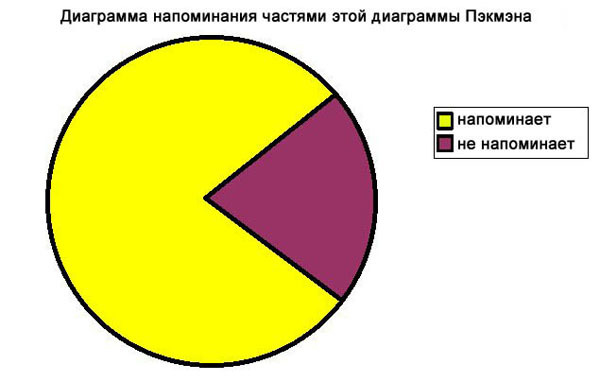
\includegraphics[scale=0.5]{Images/Pacman.jpg}
        \caption{Частка кругових діаграм, які схожі на Пекмена}
        \label{fig_pacman}
\end{figure}

\chapconclude{\ref{chap:theory}}

Наприкінці розділу знову наводяться коротенькі підсумки.